\section{Workflow}
During the projects initial phase much of the time was put on familiarizing with the ProMoVis and JModelica enviroments and the math that acts as a foundation for the Modelica models. During these first weeks there were sporadic meetings and discussions with the supervisor whenever problems or questions appeared. After an initial meeting with the developer of the ProMoVis frontend (See Appendix \ref{appC}). The start of the development of a first "Proof of concept" was initiated. After finishing this, a more thorough design phase started where both the developers of ProMoVis and a "test-user" got involved in the the process. 
\section{Tools}
\subsection{Modelica}
Modelica is a object-oriented declarative programming language used to create models of physical system. Unlike many other modelling languages, Modelica is not domain specific and thus can be used to model physical systems consisting of a mix of electrical, mechanical and chemical processes. Since the release of the first language specification in 1997 the continuous development of the language has been maintained by the Modelica Association and the current version of the Language specification is 3.2 \cite{ModelicaSpec}.\nocite{*}
\subsection{JModelica}
There is several environments, both proprietary and open source, that provides tools for compilation, analysis and simulation of  models described in Modelica. Since the use of proprietary software would demand that we separate the export tool from ProMoVis. An initial demand on the environment to be used was that it should be open source. After examining the options available JModelica\cite{jmodelicaorg}\nocite{*} was choosen because of its Python front-end, that makes it easy to interface with the tool from other software while still providing a structured environment around which we can build all parts of the export tool.   
\subsection{Numpy and SciPy}
Another important feature supporting the use of the JModelica platform was its tight integration with the NumPy and SciPy packages \cite{scipyorg}\nocite{*}. These are two very popular open source packages for Python providing a strong and well documented toolbox for mathematical computing. When extracting the mathematical models through JModelica they are represented using the data-structures provided by NumPy and in many cases this removes the need to "reinvent the wheel" for many of the operations that needs to be performed on the mathematical models before export. Instead one can directly use existing methods provided by SciPy and NumPy. The use of this package also makes the source-code for the export tool more accesible to other programmers familiar with Python and these packages.
\subsection{The SFG}
Since the SFG is a fundamental concept in ProMoVis it is motivated to give a brief introduction to how it is used in ProMoVis. ProMoVis bases its analysis and visualisation on SFG representations of dynamical systems. It is this representation the tool needs to be able to accurately extract from the existing Modelica models. Basically the an SFG is a directed graph with the vertices representing each of the states in the systems and the edges representing the relation, in terms of transfer functions, between the vertices.\\\newline The simple two tank system in Fig.~\ref{fig:twotank} Can be described by the general equations.

\begin{figure}

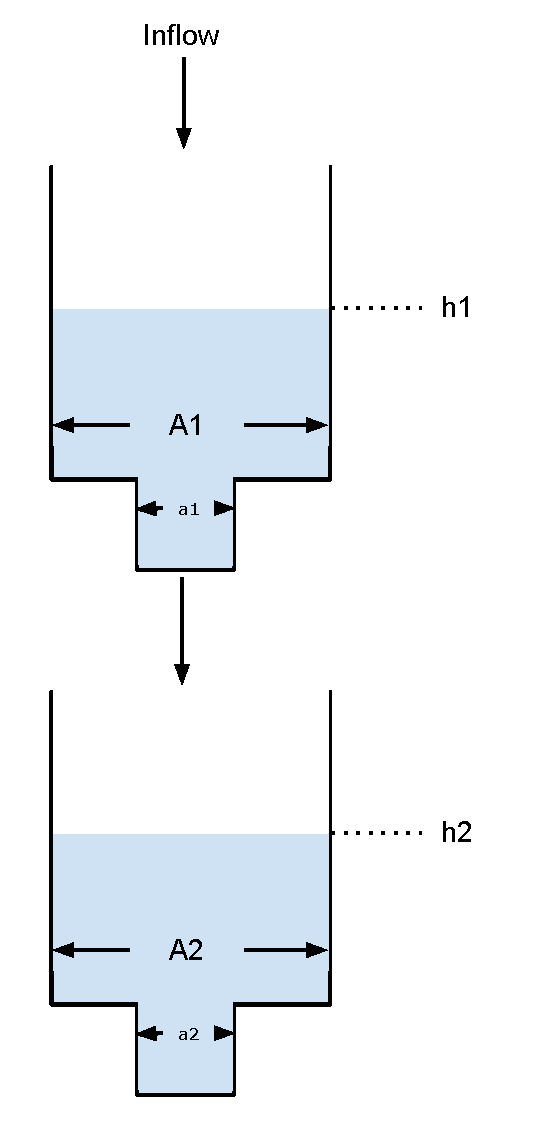
\includegraphics[scale=0.4,bb=0 0 3.67in 7.47in] {Figures/TwoTankSystem.pdf}\\\newline
\caption{A simple two tank system}
\label{fig:twotank}
\end{figure}
\begin{equation}
    \dot{h_1} = -a_1/A_1*\sqrt{2*g*h_1} + inflow\\\newline
\end{equation}
\begin{equation}
	\dot{h_2} = -a_2/A_2*\sqrt{2*g*h_2} + a_1/A_1*\sqrt{2*g*h_1}
\end{equation}
Linearising the specific model, described in Modelica,  in Appendix \ref{appD}. We can then extract the transfer functions. For the parameters specified the following is obtained:\\\newline
Transfer function from inflow to h1 is : $\begin{array}{rcl} \frac{1}{s +2.3*10^{-2}} \end{array}$\\\newline
Transfer function from h1 to h2 is :$\begin{array}{rcl} \frac{2.3*10^{-2}}{s +8.9*10^{-2}} \end{array}$\\\newline
And the corresponding signal flow graph, as shown in Fig.~\ref{fig:sfg}, can be obtained. From the figure, it is easy to see that the vertices in the SFG is the states of the system and the edges are the transfer functions between the states. In ProMoVis, there is also additional information supplied with the vertices, such as operating point, saturation values etc. 
\begin{figure}
\fbox{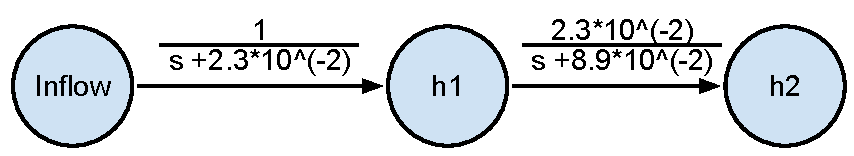
\includegraphics[scale=0.8,bb=0 0 5.69in 1.04in] {Figures/sfgtwotank.pdf}}
\caption{Corresponding SFG for the two tank system in Fig~\ref{fig:twotank}}
\label{fig:sfg}
\end{figure}
